%%%%%%%%%%%%%%%%%%%%%%%%%%%%%%%%%%%%
% Header                           %
%%%%%%%%%%%%%%%%%%%%%%%%%%%%%%%%%%%%
% 
% Revisions: 2017-04-10 Martin Rädel <martin.raedel@dlr.de>
%                       Initial draft
%               
% Contact:   Martin Rädel,  martin.raedel@dlr.de
%            DLR Composite Structures and Adaptive Systems
%          
%                                 __/|__
%                                /_/_/_/  
%            www.dlr.de/fa/en      |/ DLR
% 
%%%%%%%%%%%%%%%%%%%%%%%%%%%%%%%%%%%%
% Content                          %
%%%%%%%%%%%%%%%%%%%%%%%%%%%%%%%%%%%%

% \section{Description}
\leveldown{Description}

\marktool[\tooladdress]{\toolnameshort} is an open-source computational peridynamics code developed at Sandia National Laboratories for massively-parallel multi-physics simulations.  It has been applied primarily to problems in solid mechanics involving pervasive material failure.  \marktool[\tooladdress]{\toolnameshort} is a \Cpp{} code utilizing foundational software components from Sandia's \marktool{Trilinos} project and is fully compatible with the Cubit mesh generator and \marktool[\paraviewname]{\paraviewname} visualization code.

\marktool[\tooladdress]{\toolnameshort} development began under the Physics \& Engineering Models element of the US DOE's Advanced Simulation and Computing (ASC) program.  The project was led by Michael Parks and managed by John Aidun.  Subsequent funding has been provided by the US DOE through the ASC, ASCR, and LDRD programs.

\levelstay{Adresses}

{
\renewcommand{\arraystretch}{1.3}
\begin{tabularx}{\linewidth}{@{}lX}
Official homepage:      & \href{https://peridigm.sandia.gov/}{https://peridigm.sandia.gov/}\\
Source code repository: & \href{https://github.com/peridigm/peridigm}{https://github.com/peridigm/peridigm}\\
Release snapshots:      & Must be requested via Download Registration Form on \href{https://peridigm.sandia.gov/content/download-registration-form}{https://peridigm.sandia.gov/content/download-registration-form}\\
User guide \cite{PeridigmUserGuide100}:& \href{http://www.sandia.gov/~djlittl/docs/PeridigmV1.0.0.pdf}{http://www.sandia.gov/~djlittl/docs/PeridigmV1.0.0.pdf}
\end{tabularx}
}

\levelstay{Hardware requirements}

Currently, there are no hardware requirements available or known. Publications, reports and presentations continuously mention the massive parallelization possbile and presumably also necessary to run \marktool[\tooladdress]{\toolnameshort}.

Information on the performance of \marktool[\tooladdress]{\toolnameshort} on different system will be added as soon as it is available.

% \section{Features}
\levelstay{Features}

% \subsection{Example 1}
\leveldown{Example 1}

\begin{wrapfigure}[7]{r}{5.0cm}
% \raisebox{0pt}[\dimexpr\height-0.6\baselineskip\relax]{
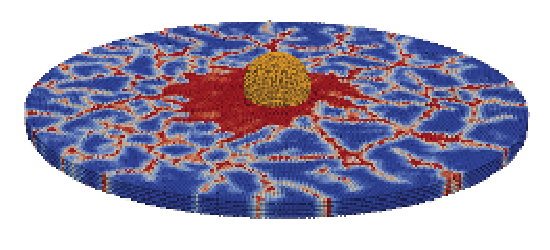
\includegraphics[width=5.0cm]{Figures/Peridigm_slide-image-1}
% }
% \caption{Brittle impact failure}
\caption{Impact failure}
\label{fig:Peridigm_Ex1}
\end{wrapfigure}

The simulation of impact and brittle fracture displayed \autoref{fig:Peridigm_Ex1} was achieved using explicit transient dynamics, the linear peridynamic solid constitutive model, short-range force contact, and a critical stretch bond failure law. \par Peridynamics provides a natural framework for capturing pervasive material failure and fracture.

% \subsection{Example 2}
\levelstay{Example 2}

\marktool[\tooladdress]{\toolnameshort} is capable of performing explicit dynamic, implicit dynamic, and quasi-static time integration.

\begin{wrapfigure}[4]{r}{5.0cm}
% \raisebox{0pt}[\dimexpr\height-0.6\baselineskip\relax]{

\includegraphics[width=5.0cm]{Figures/Peridigm_slide-image-2}
% }
% \caption{Brittle impact failure}
\caption{Tensile test}
\label{fig:Peridigm_Ex2}
\end{wrapfigure}

The tensile test simulation presented in \autoref{fig:Peridigm_Ex2} was attained using an elastic correspondence constitutive model and quasi-static time integration. Pre- and post-processing were carried out using Sandia's \marktool{Cubit} mesh generator and \marktool{ParaView} visualization code.

% \subsection{Example 3}
\levelstay{Example 3}

\begin{wrapfigure}[8]{r}{5.0cm}
\centering
\raisebox{0pt}[\dimexpr\height-0.7\baselineskip\relax]{
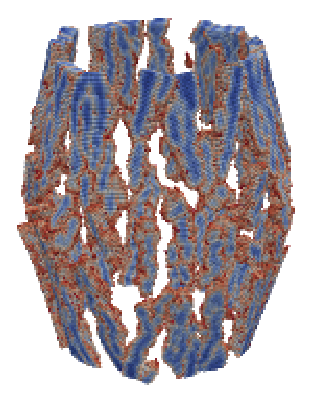
\includegraphics[width=3.5cm]{Figures/Peridigm_slide-image-3}
}
% \caption{Brittle impact failure}
\caption{Fragmentation}
\label{fig:Peridigm_Ex3}
\end{wrapfigure}

The fragmentation of an expanding cylinder, shown in \autoref{fig:Peridigm_Ex3}, was simulated using the linear peridynamic solid constitutive model and critical-stretch bond failure rule. Initial velocities for each node in the discretization were specified via user-supplied analytic expressions.

\toolnameformatted utilizes the RTCompiler function parser to process C-style expressions for the specification of input parameters, including initial and boundary conditions.

% \section{License}
\levelup{License}

As of 04.02.2016 \marktool[\tooladdress]{\toolnameshort} is distributed under the three-term BSD license.

The current license terms can be obtained from:\\ \url{https://peridigm.sandia.gov/content/license}.

% \section{\toolname working environment}
\levelstay{\toolname{} working environment}

\marktool[\tooladdress]{\toolnameshort} is a standalone tool for the handling of peridynamic models. Sandia National Labs suggests the use of \marktool[\cubitaddress]{\cubitname} as the mesh generator and pre-processor and \marktool[\paraviewname]{\paraviewname} for post-processing. However, \marktool[\cubitaddress]{\cubitname} is not publicly available free of charge except for U.S. government agencies. Any visualization package capable of reading and displaying ExodusII-format \cite{ExodusII1994} data may be used to
visualize the output of a Peridigm simulation. The creators of \marktool[\tooladdress]{\toolnameshort} use \marktool[\paraviewname]{\paraviewname}.

This installation guide focusses on the installation of the core program \marktool[\tooladdress]{\toolnameshort}. Several libraries are required as well as some basic tools \marktool[\tooladdress]{\toolnameshort} or one of its libraries is dependent on. All required tools for the use of \marktool[\tooladdress]{\toolnameshort} in a working environment are shown in \autoref{fig:Peridigm_working_environment}.

\begin{figure}[htbp]
\small
\footnotesize
\centering
\begin{tikzpicture}[
% for small:
%     level distance=1.5cm,
%     level 1/.style={sibling distance=4cm},
%     level 2/.style={sibling distance=1.5cm},
%     level 3/.style={sibling distance=5.75cm},
%     level 4/.style={sibling distance=1.4cm},
%     level 5/.style={sibling distance=1.2cm},
% for footnotesize:
	level distance=1.5cm,
	level 1/.style={sibling distance=4cm},
	level 2/.style={sibling distance=1.5cm},
	level 3/.style={sibling distance=6.5cm},
	level 4/.style={sibling distance=1.75cm},
	level 5/.style={sibling distance=1.0cm},
  ]
  \node {Peridigm environment}
	child[color=gray] {node {Preprocessing}
	  child {node {\marktool[\cubitaddress]{\cubitname} mesh generator}}
	}
	child {node {Solution}
	  child {node {\marktool[\tooladdress]{\toolnameshort}}
	child {node {Basics}
	  child {node {Compiler}
	    child {node {Fortran}}
	    child {node {C}}
	    child {node {\Cpp}}
	  }
	  child {node {\marktool[\cmakeaddress]{\cmakename}}}
	  child {node {MPI}
	    %child {node {\marktool[\openmpiaddress]{\openmpiname}}}
	    %child {node {\marktool[\mpichaddress]{\mpichname}}}
	  }
	  child {node {\marktool[\pythonaddress]{\pythonname}}}
	}
	child {node {Libraries}
	  child {node[color=gray] {\marktool[\boostaddress]{\boostname}}}
	  child {node {\marktool[\netcdfaddress]{\netcdfname}}
	    child {node {\marktool{m4}}}
	  }
	  child {node {\marktool[\hdfaddress]{\hdfname}}}
	  child {node {\marktool[\trilinosaddress]{\trilinosname}}
	    child {node {\marktool{BLAS}}}
	    child {node {\marktool{LAPACK}}}
	    child {node {\marktool{X11}}}
	    child {node {\marktool{yaml}}}
	  }
	}
	  }
	}
	child {node {Postprocessing}
	  child {node {Vtk/\marktool[\paraviewname]{\paraviewname}}}
	};
\end{tikzpicture}
\caption{\toolname{} working environment tree}
\label{fig:Peridigm_working_environment}
\end{figure}

The installation guide features descriptions to the installation of all basic tools, libraries and \marktool[\tooladdress]{\toolnameshort} itself.

\levelstay{Dependencies}

Below the dependencies between the individual tools and packages are shown.

\begin{figure}[htbp]
\small
% \footnotesize
\centering
\newcommand\irad{4cm}
\newcommand\orad{6cm}
\begin{tikzpicture}
% Tools
\draw (1*360/9:\irad) node (Compiler) {Compiler};
\draw (2*360/9:\irad) node (CMake)    {\cmakename};
\draw (3*360/9:\irad) node[align=center] (MPI)      {MPI\\(-Compiler)};
\draw (4*360/9:\irad) node (Python)   {\pythonname};
\draw (5*360/9:\irad) node[color=gray] (Boost)    {\boostname};
\draw (6*360/9:\irad) node (HDF5)     {\hdfname};
\draw (7*360/9:\irad) node (NetCDF)   {\netcdfname};
\draw (8*360/9:\irad) node (Trilinos) {\trilinosname};
\draw (9*360/9:\irad) node (Peridigm) {\toolname};
% Zusatztools
\draw (7.75*360/9:\orad) node (BLAS)   {BLAS};
\draw (8.00*360/9:\orad) node (LAPACK) {LAPACK};
\draw (8.25*360/9:\orad) node (X11)    {X11};
\draw (8.50*360/9:\orad) node (yaml)   {yaml};
%
\draw (7*360/9:\orad) node (m4)   {m4};
% Striche
\draw[-latex] (BLAS)   -- (Trilinos);
\draw[-latex] (LAPACK) -- (Trilinos);
\draw[-latex] (X11)    -- (Trilinos);
%
\draw[-latex] (m4)   -- (NetCDF);
%
\draw[-latex] (Compiler) -- (CMake);
\draw[-latex] (Compiler) -- (MPI);
% \draw[-latex] (Compiler) -- (Boost);
% \draw[-latex] (Compiler) -- (HDF5);
% \draw[-latex] (Compiler) -- (NetCDF);
% \draw[-latex] (Compiler) -- (Trilinos);
% \draw[-latex] (Compiler) -- (Peridigm);
%
\draw[-latex] (Python) -- (Peridigm);
%
\draw[-latex] (CMake) -- (Trilinos);
\draw[-latex] (CMake) -- (Peridigm);
%
\draw[-latex] (MPI) -- (Boost);
\draw[-latex] (MPI) -- (HDF5);
\draw[-latex] (MPI) -- (NetCDF);
\draw[-latex] (MPI) -- (Trilinos);
\draw[-latex] (MPI) -- (Peridigm);
%
\draw[-latex] (HDF5)   -- (NetCDF);
\draw[-latex] (HDF5)   -- (Trilinos);
\draw[-latex] (Boost)  -- (Trilinos);
\draw[-latex] (NetCDF) -- (Trilinos);
\draw[-latex] (yaml)   -- (Trilinos);
%
\draw[-latex] (Boost)    -- (Peridigm);
\draw[-latex] (Trilinos) -- (Peridigm);
\end{tikzpicture}
\caption{\toolname{} package dependencies}
\label{fig:Peridigm_dependencies}
\end{figure} 
